\begin{frame}
  \frametitle{Control Rods in MSRs}
  \begin{columns}
    \hfill
    \column[t]{5cm}
    \vspace{.2cm}
    \begin{figure}
      \centering
      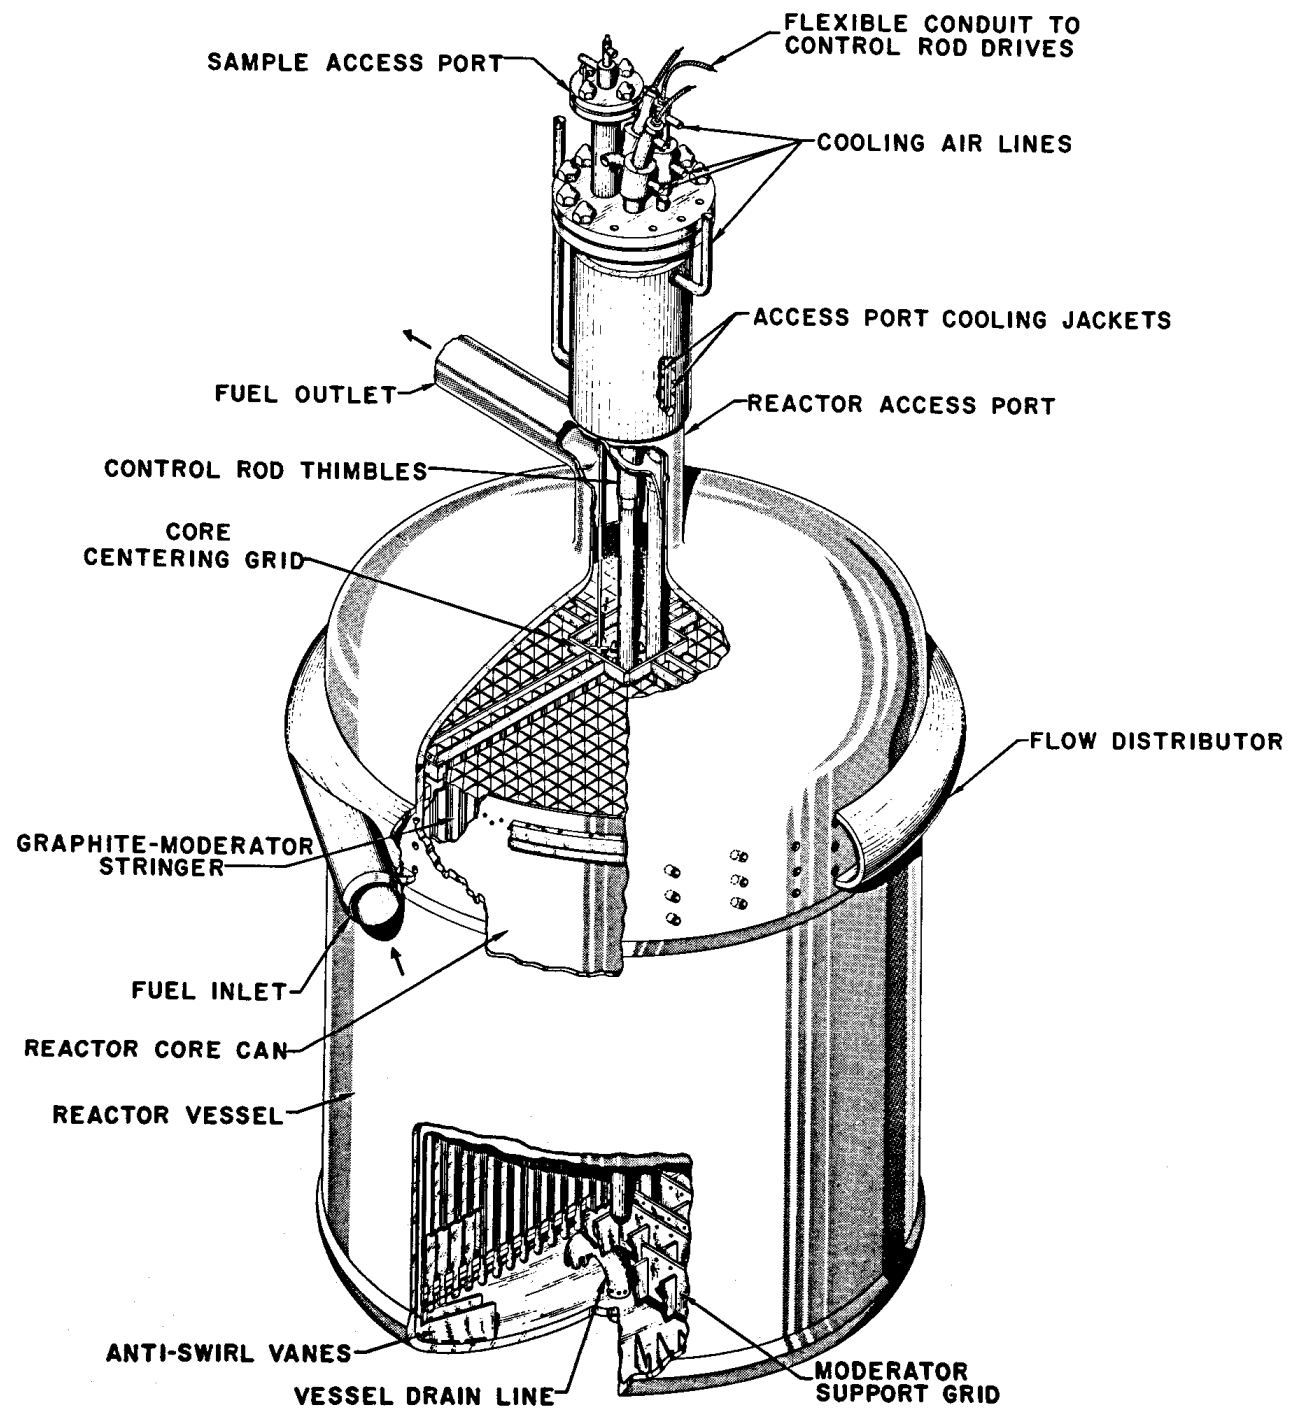
\includegraphics[width=\columnwidth]{images/msre-cutout}
      \caption{\footnotesize MSRE reactor vessel \cite{robertson_msre_1965}}
    \end{figure}
    \hfill
    \column[t]{6cm}
    \begin{figure}
      \centering
      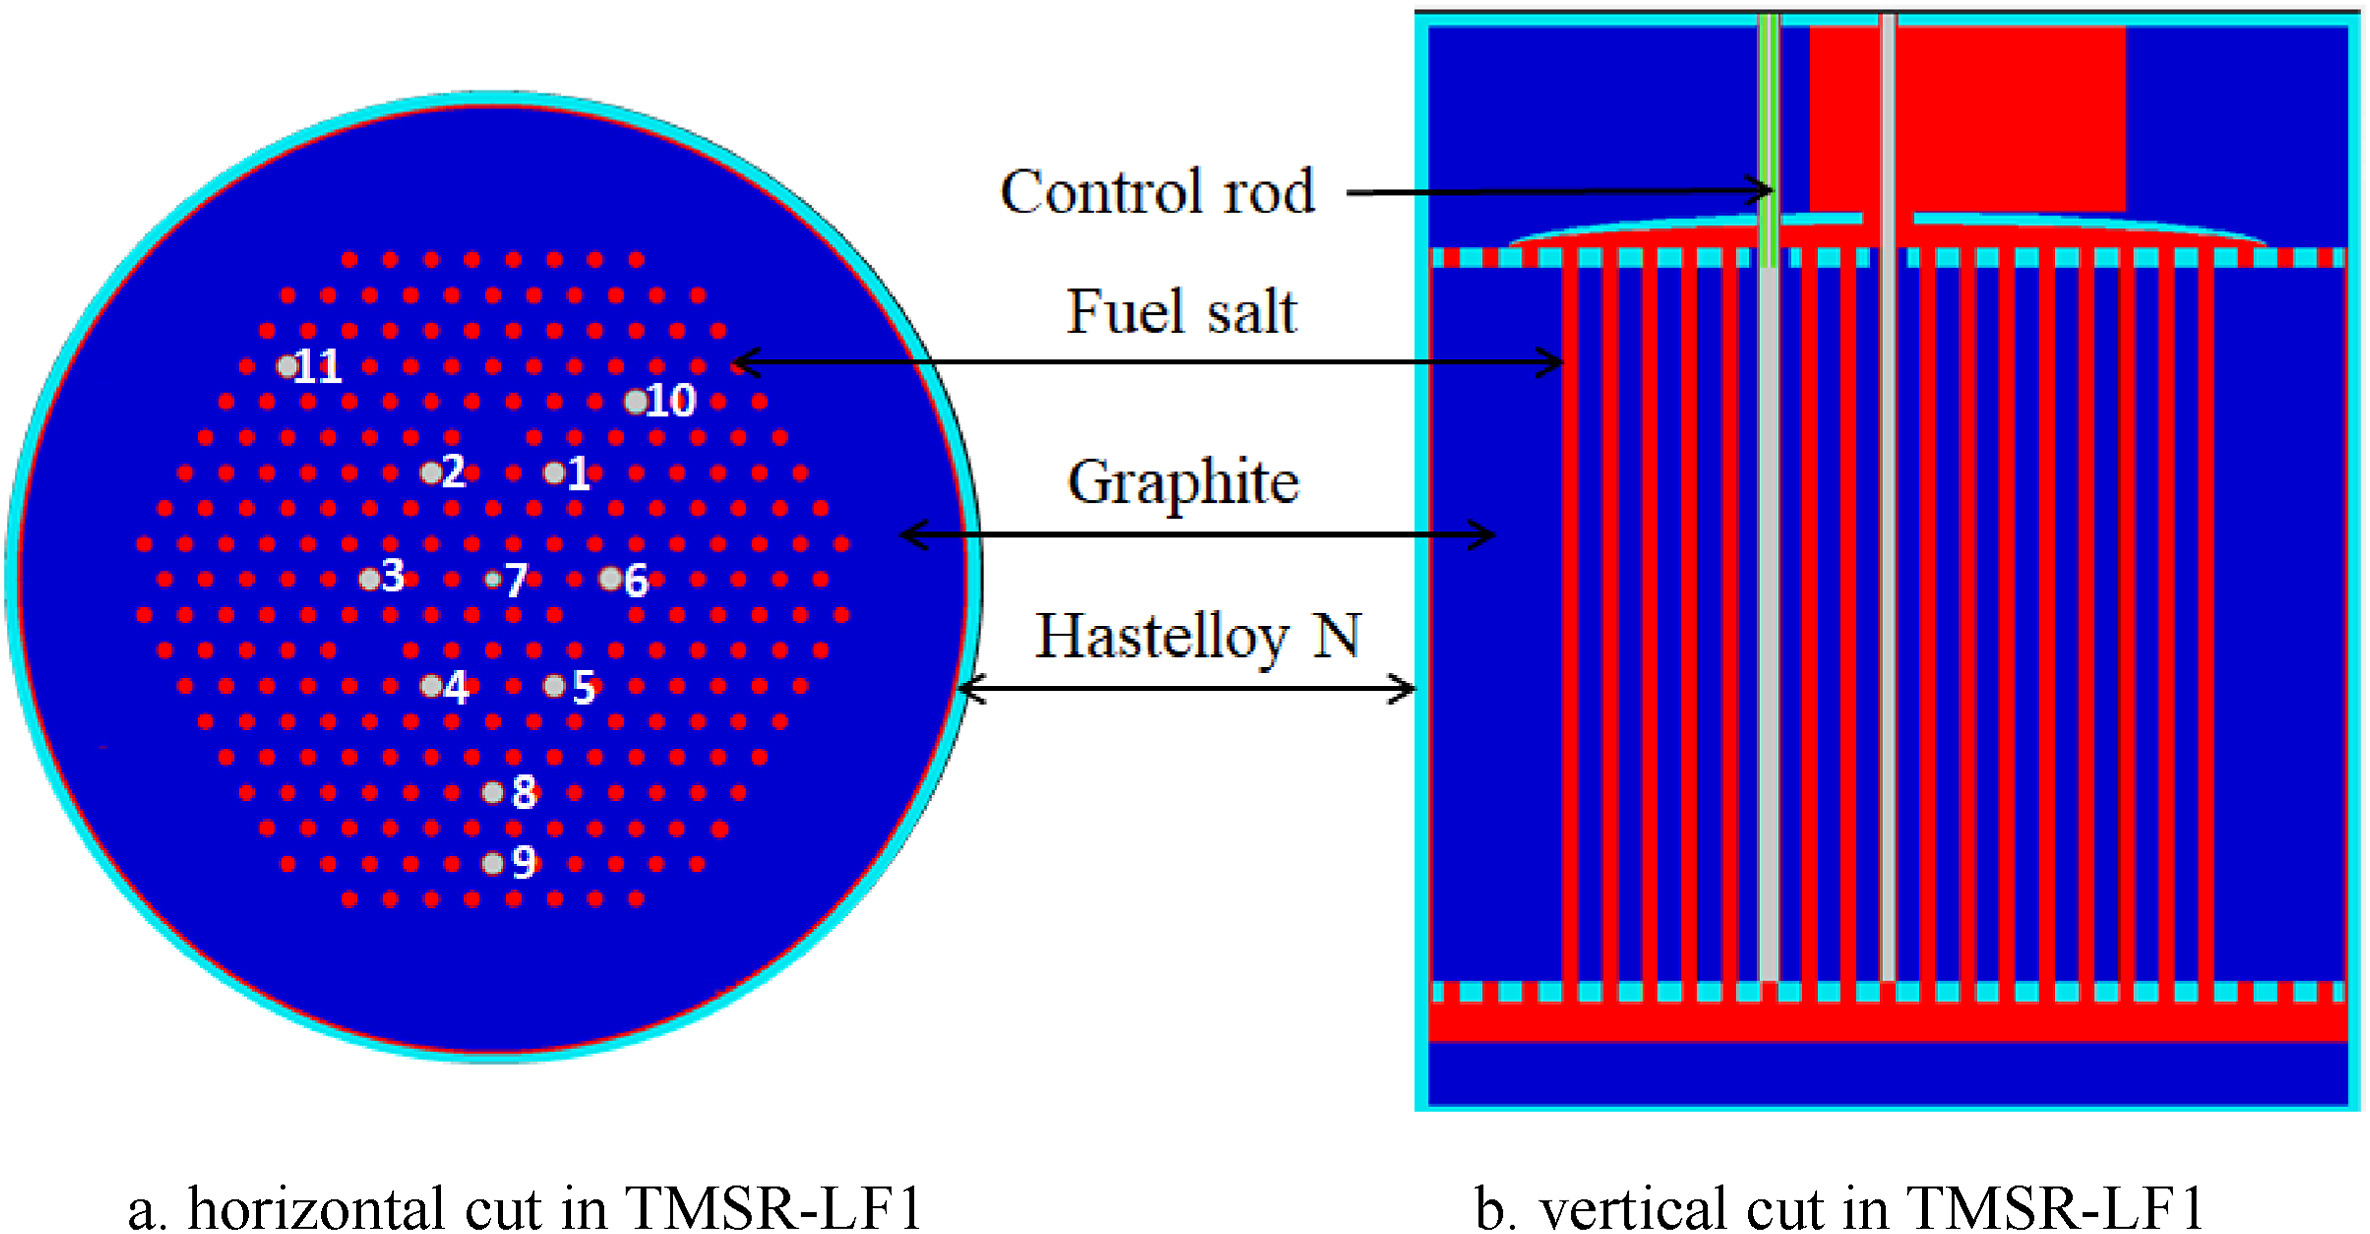
\includegraphics[width=.8\columnwidth]{images/tmsr}
      \caption{\footnotesize Cross-sectional views of the TMSR-LF1
      \cite{liu_sensitivityuncertainty_2020}}
    \end{figure}
    \begin{figure}
      \centering
      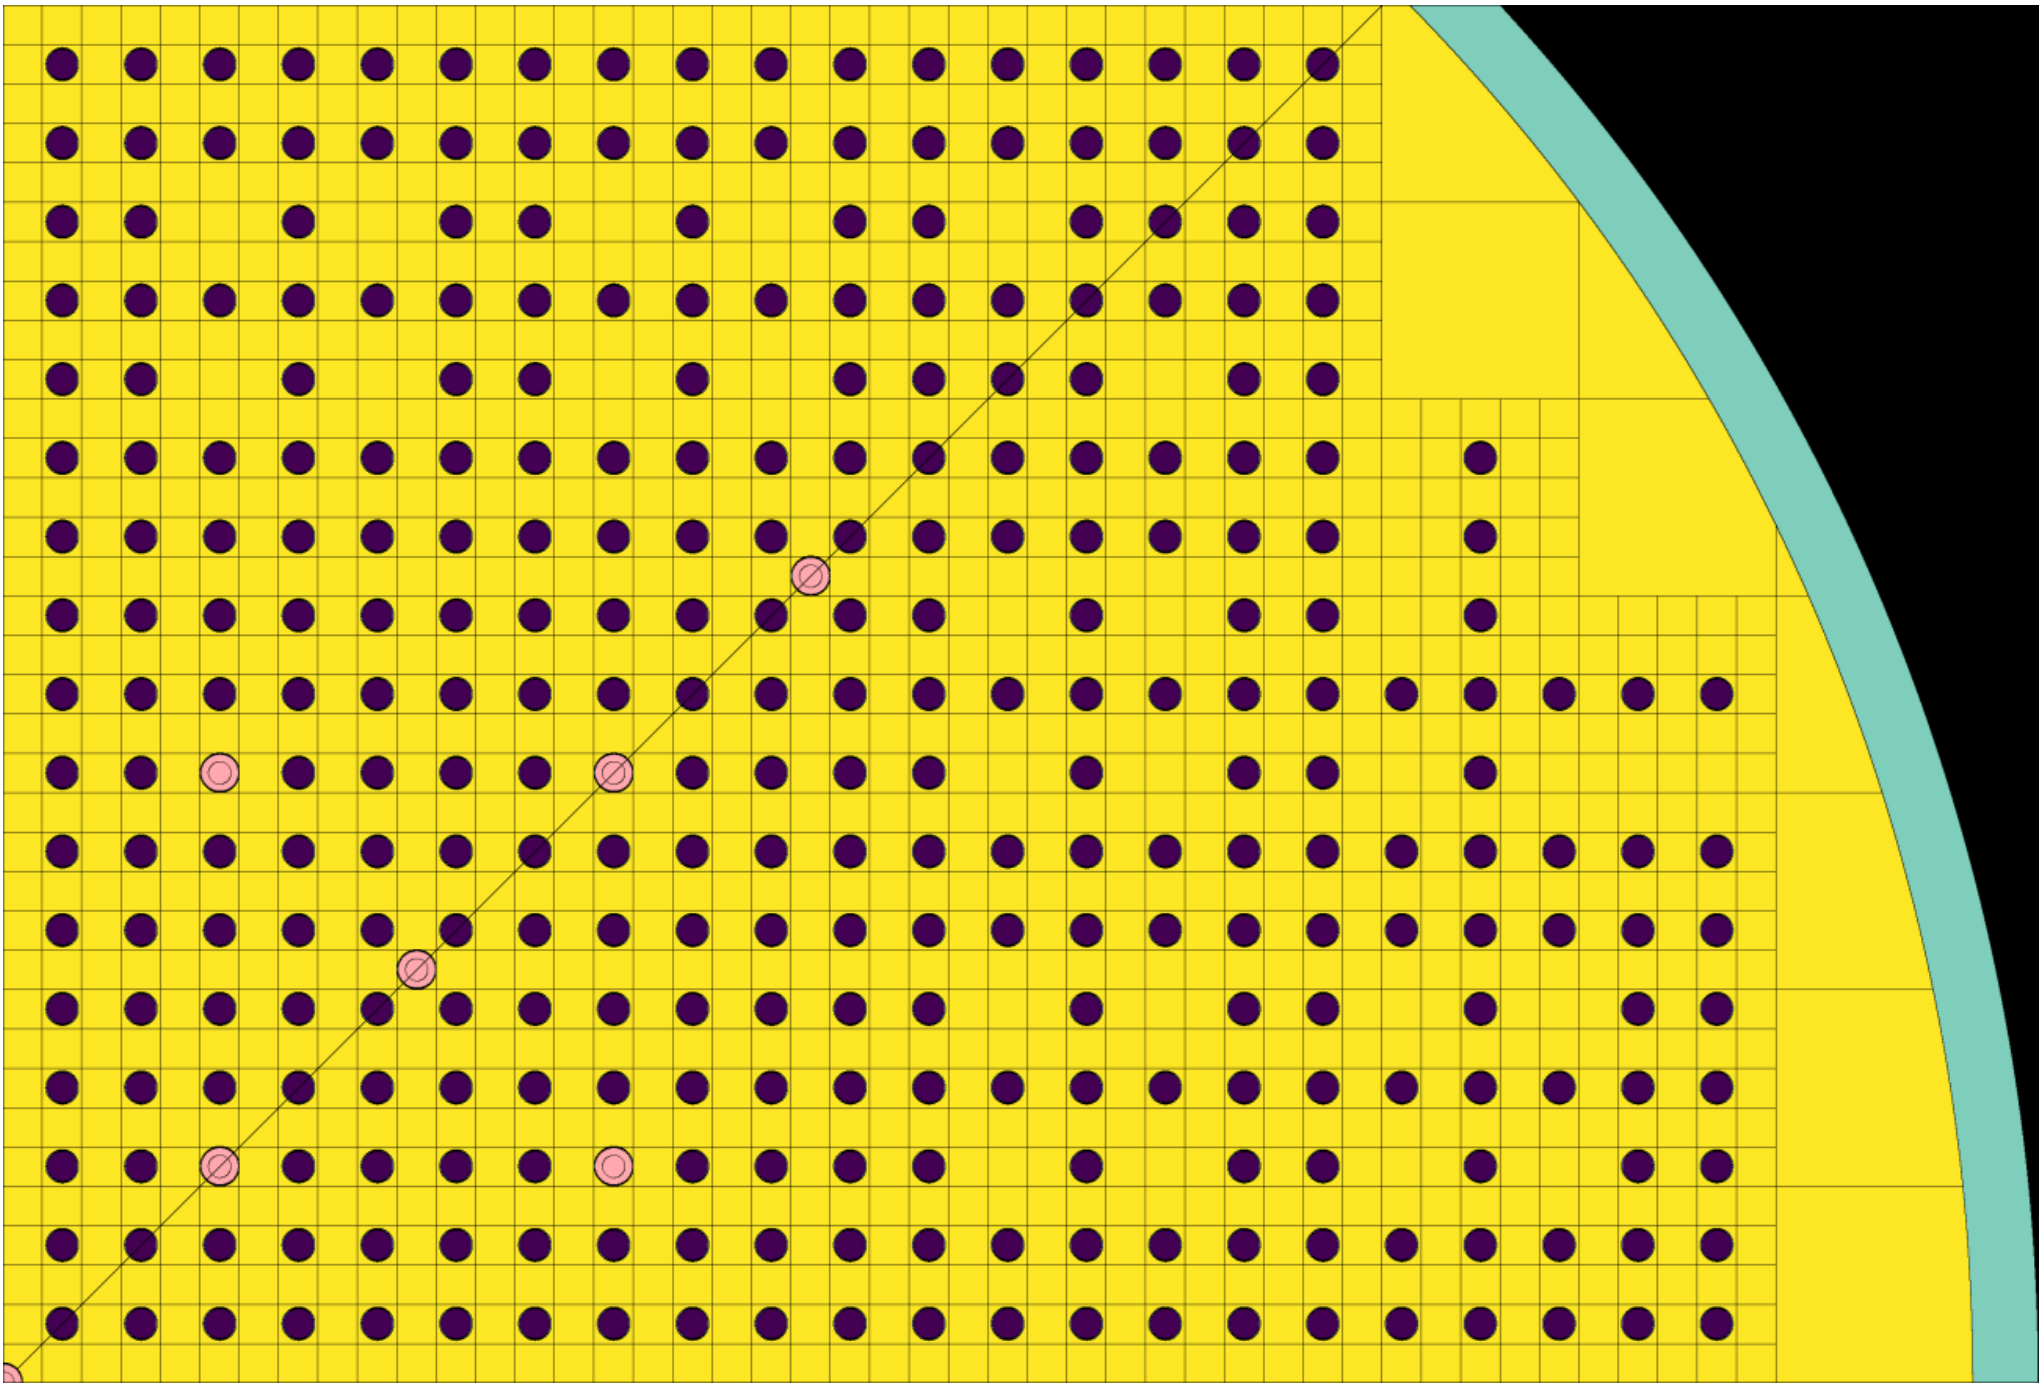
\includegraphics[width=.5\columnwidth]{images/tap-msr-rods}
      \caption{\footnotesize Cross-sectional view of the TAP MSR \cite{lee_neutronics_2020}}
    \end{figure}
    \hfill
  \end{columns}
\end{frame}

\begin{frame}
  \frametitle{Control Rods in MSRs}
  \textbf{Control rods provide a means of controlling the fission rate in nuclear reactors.} 
  \begin{itemize}
    \item Facilitate reactor start-up, shut-down, or load-following operations
    \item Consist of highly neutron-absorbing materials such as boron or gadolinium
  \end{itemize}
  \textbf{Control rods are also important for licensing and safety characterization.}

  $\Rightarrow$ \textbf{It is important to characterize control rod effects in all relevant
  transient scenarios.}
%  \textbf{Many MSR designs contain comparatively fewer control rods than most other reactor types due to:}
%  \begin{itemize}
%    \item Uniform liquid fuel burnup
%    \item Strong passive safety of the liquid fuel form
%    \item Low excess reactivity of fuel inventory
%    \item Availability of other control mechanisms
%  \end{itemize}

\end{frame}

\begin{frame}
  \frametitle{Control Rod Modeling}
  \textbf{Control rods induce highly anisotropic neutron fluxes and steep flux gradients in their
  vicinity.}
  \begin{block}{\textbf{The Control Rod Modeling Dilemma}}
    \begin{itemize}
      \item Neutron diffusion, $P_1$, and $SP_N$ methods perform poorly near control rod regions
        due to the highly anisotropic neutron fluxes and steep flux gradients
      \item High-fidelity neutron transport methods remain too computationally expensive for
        routine time-dependent multiphysics simulations
    \end{itemize}
  \end{block}
\end{frame}

\begin{frame}
  \frametitle{Control Rod Modeling in MSR Multiphysics Studies}
  \vspace{.2cm}

  Common approximations applied to control rod modeling include:
  \begin{itemize}
    \item Homogenized, coarse-mesh geometries containing static control rods with albedo neutron
      flux boundary conditions \cite{kophazi_development_2009} or transport-corrected cross
      sections \cite{cui_development_2021, jaradat_development_2021, yang_development_2022}
      \begin{itemize}
        \item Neutronics geometry differs from thermal-hydraulics geometry
        \item Static calibration factors may not be suitable for time-dependent simulations
      \end{itemize}
    \item Scaling the neutron source term to simulate moving control rods
      \cite{delpech_benchmark_2003, krepel_dyn3d-msr_2007, jaradat_development_2021,
      yang_development_2022}
      \begin{itemize}
        \item Does not capture local or asymmetric flux changes
      \end{itemize}
  \end{itemize}

  \begin{block}{\textbf{Technical Gap}}
    \textbf{There are no MSR simulation tools or studies that explicitly model moving control rods.}
  \end{block}
\end{frame}
